\documentclass{article}

% Packages forked from the original template
\usepackage{fancyhdr}
\usepackage{extramarks}
\usepackage{amsmath}
\usepackage{amsthm}
\usepackage{amsfonts}
\usepackage{tikz}
\usepackage[plain]{algorithm}
\usepackage{algpseudocode}

% Extra packages
\usepackage{changepage} % adjustwidth environment
\usepackage{hyperref} % href
\usepackage{xcolor} % colored text
\usepackage{enumerate}
\usepackage{graphicx}

\usetikzlibrary{automata,positioning}

% Additional commands
\def\eg{\emph{e.g., }}
\def\ie{\emph{i.e., }}
\def\cf{\emph{c.f., }}
\def\etc{\emph{etc. }}
\def\wrt{\emph{w.r.t. }}
\def\etal{\emph{et al. }}

%
% Basic Document Settings
%

\topmargin=-0.45in
\evensidemargin=0in
\oddsidemargin=0in
\textwidth=6.5in
\textheight=9.0in
\headsep=0.25in

\linespread{1.1}

\pagestyle{fancy}
\lhead{\hmwkClass: \hmwkTitle}
\rhead{\firstxmark}
\lfoot{\lastxmark}
\cfoot{\thepage}

\renewcommand\headrulewidth{0.4pt}
\renewcommand\footrulewidth{0.4pt}

\setlength\parindent{0pt}

%
% Create Problem Sections
%

\newcommand{\enterProblemHeader}[1]{
    \nobreak\extramarks{}{Exercise \arabic{#1} continued on next page\ldots}\nobreak{}
    \nobreak\extramarks{Exercise \arabic{#1} (continued)}{Exercise \arabic{#1} continued on next page\ldots}\nobreak{}
}

\newcommand{\exitProblemHeader}[1]{
    \nobreak\extramarks{Exercise \arabic{#1} (continued)}{Exercise \arabic{#1} continued on next page\ldots}\nobreak{}
    \stepcounter{#1}
    \nobreak\extramarks{Exercise \arabic{#1}}{}\nobreak{}
}

\setcounter{secnumdepth}{0}
\newcounter{partCounter}
\newcounter{homeworkProblemCounter}
\setcounter{homeworkProblemCounter}{1}
\nobreak\extramarks{Exercise \arabic{homeworkProblemCounter}}{}\nobreak{}

%
% Homework Problem Environment
%
% This environment takes an optional argument. When given, it will adjust the
% problem counter. This is useful for when the problems given for your
% assignment aren't sequential. See the last 3 problems of this template for an
% example.
%
\newenvironment{homeworkProblem}[1][-1]{
    \ifnum#1>0
        \setcounter{homeworkProblemCounter}{#1}
    \fi
    \section{Exercise \arabic{homeworkProblemCounter}}
    \setcounter{partCounter}{1}
    \enterProblemHeader{homeworkProblemCounter}
}{
    \exitProblemHeader{homeworkProblemCounter}
}

%
% Homework Details
%   - Title
%   - Due date
%   - Class
%   - Section/Time
%   - Instructor
%   - Author
%

\newcommand{\hmwkTitle}{Assignment 12}
\newcommand{\hmwkDueDate}{July 16, 2024}
\newcommand{\hmwkClass}{Continuous Optimization}
\newcommand{\hmwkAuthorName}{ \textbf{Honglu Ma} \and \textbf{Hiroyasu Akada} \and \textbf{Mathivathana Ayyappan}}

%
% Title Page
%

\title{
    \vspace{2in}
    \textmd{\textbf{\hmwkClass:\ \hmwkTitle}}\\
    \normalsize\vspace{0.1in}\small{Due\ on\ \hmwkDueDate}\\
    \vspace{3in}
}

\author{\hmwkAuthorName}
\date{}

\renewcommand{\part}[1]{\textbf{\large Part \Alph{partCounter}}\stepcounter{partCounter}\\}

%
% Various Helper Commands
%

% Useful for algorithms
\newcommand{\alg}[1]{\textsc{\bfseries \footnotesize #1}}

% For derivatives
\newcommand{\deriv}[1]{\frac{\mathrm{d}}{\mathrm{d}x} (#1)}

% For partial derivatives
\newcommand{\pderiv}[2]{\frac{\partial}{\partial #1} (#2)}

% Integral dx
\newcommand{\dx}{\mathrm{d}x}

% Alias for the Solution section header
\newcommand{\solution}{\textbf{\large Solution}}

% Probability commands: Expectation, Variance, Covariance, Bias
\newcommand{\E}{\mathrm{E}}
\newcommand{\Var}{\mathrm{Var}}
\newcommand{\Cov}{\mathrm{Cov}}
\newcommand{\Bias}{\mathrm{Bias}}

% Norm
\newcommand{\norm}[1]{\left\lVert#1\right\rVert}

% Margined Homework Subsection
\newenvironment{homeworkSubsection}[1]{%
    \subsection*{#1}%
    \begin{adjustwidth}{2.5em}{0pt}%
}{%
    \end{adjustwidth}%
}

\begin{document}

\maketitle

\pagebreak

\begin{homeworkProblem}[1]
    \begin{homeworkSubsection}{1}
        \begin{enumerate}[(i)]
            \item Not convex. Consider $p = 3$ we have $f(x) = x^3$ and $f''(x) = 6x \leq 0$ when $x \leq 0$.
            \item Convex. $f''(x) = x^{-2} \geq 0$
            \item Convex. $f''(x) = \alpha^2 e^{\alpha x} \geq 0$
            \item Convex. $f''(x) = \frac{1}{(1-x)} \geq 0$ when $x \in (0, 1)$
        \end{enumerate}
    \end{homeworkSubsection}
    \begin{homeworkSubsection}{2}
        \begin{enumerate}[(i)]
            \item Convex. 
            
            Take $x, y \in C$. 

            Consider $||(1-\lambda)x+\lambda y||_2 \overset{Cauchy-Schwarz}{\leq} ||(1-\lambda)x||_2 + ||\lambda y||_2 = (1-\lambda)||x||_2 + \lambda||y||_2 \leq 1$.
            \item Not convex. Consider
            $x = \begin{pmatrix}
                0 \\ 1 
            \end{pmatrix}$, 
            $y = \begin{pmatrix}
                1 \\ 0 
            \end{pmatrix}$
            and $\lambda = \frac{1}{2}$.

            Clearly $||(1-\lambda)x + \lambda y||_2 = \frac{\sqrt{2}}{2}\neq 1$.
            \item Not convex. Consider
            $x = \begin{pmatrix}
                1 \\ 1 
            \end{pmatrix}$, 
            $y = \begin{pmatrix}
                -1 \\ -1
            \end{pmatrix}$
            and $\lambda = \frac{1}{2}$.

            Clearly $||(1-\lambda)x + \lambda y||_{\infty} = ||\begin{pmatrix}
                0 \\ 0
            \end{pmatrix}||_{\infty} = 0 \neq 1$.
            \item Convex.
            Similar to (i).
        \end{enumerate}
    \end{homeworkSubsection}
    \begin{homeworkSubsection}{3}
        See appendix
    \end{homeworkSubsection}
    \begin{homeworkSubsection}{4}
        \begin{align*}
            T_C(\begin{pmatrix}
                1 & 1
            \end{pmatrix}^\top) &= \left\{
                \begin{pmatrix}
                    x_1 \\ x_2
                \end{pmatrix} \in \mathbb{R}^2 \mid x_1 \leq 1, x_2 \leq 1
            \right\}\\
            N_C(\begin{pmatrix}
                1 & 1
            \end{pmatrix}^\top) &= \left\{
                \begin{pmatrix}
                    x_1 \\ x_2
                \end{pmatrix} \in \mathbb{R}^2 \mid x_1 \geq 1, x_2 \geq 1
            \right\}\\
        \end{align*}
    \end{homeworkSubsection}
\end{homeworkProblem}
\begin{homeworkProblem}[2]
    \begin{homeworkSubsection}{(A)}
        In steepest descent method, we have
        $x^{(k+1)} = x^{(k)} - \alpha \nabla f(x^{(k)})$.
        We can approximate $f(x^{(k+1)})$ with its second order Taylor expansion around $x^{(k)}$.
        \begin{align*}
            f(x^{(k+1)}) &\approx f(x^{(k)}) + \nabla f(x^{(k)})^\top (x^{(k+1)} - x^{(k)}) + \frac{1}{2} (x^{(k+1)} - x^{(k)})^\top \nabla^2 f(x^{(k)}) (x^{(k+1)} - x^{(k)})\\
            &= f(x^{(k)}) - \alpha \nabla f(x^{(k)})^\top \nabla f(x^{(k)}) + \frac{\alpha^2}{2} \nabla f(x^{(k)})^\top \nabla^2 f(x^{(k)}) \nabla f(x^{(k)}) =: g(\alpha)\\
        \end{align*}
        We can find the optimal $\alpha$ by solving $\frac{dg}{d\alpha} = 0$.
        \begin{align*}
            \frac{dg}{d\alpha} &= -\nabla f(x^{(k)})^\top \nabla f(x^{(k)}) + \alpha \nabla f(x^{(k)})^\top \nabla^2 f(x^{(k)}) \nabla f(x^{(k)}) = 0\\
            \nabla f(x^{(k)})^\top \nabla f(x^{(k)}) &= \nabla f(x^{(k)})^\top (\alpha\nabla^2 f(x^{(k)})) \nabla f(x^{(k)})
        \end{align*}
        By choosing $\alpha = (\nabla^2 f(x^{(k)}))^{-1}$, we can cancel the affect of rescaling of the Hessian matrix.
        
        Thus we arrive at the Newton's method: $x^{(k+1)} = x^{(k)} - (\nabla^2 f(x^{(k)}))^{-1} \nabla f(x^{(k)})$.
    \end{homeworkSubsection}
    \begin{homeworkSubsection}{(B)}
        \begin{enumerate}[Step 1]
            \setcounter{enumi}{-1}
            \item Let $x^{(0)} := \begin{pmatrix}
                0 \\ 0
            \end{pmatrix}$
            \begin{align*}
                d^{(0)} = r^{(0)}
                &= -\nabla f(x^{(0)})\\
                &= -b - Qx^{(0)}\\
                &= -\begin{pmatrix}
                    1 \\ -1
                \end{pmatrix}
                - \begin{pmatrix}
                    4 & 3\\
                    3 & 6
                \end{pmatrix}\begin{pmatrix}
                    0 \\ 0
                \end{pmatrix}\\
                &= \begin{pmatrix}
                    -1 \\ 1
                \end{pmatrix}\\
                \tau_0 &= \frac{\langle r^{(0)}, r^{(0)}\rangle}{\langle d^{(0)}, Qd^{(0)}\rangle}\\
                &= \frac{1}{2}
            \end{align*}
            \item 
            \begin{align*}
                x^{(1)} &= x^{(0)} + \tau_0 d^{(0)}\\
                &= \begin{pmatrix}
                    0 \\ 0
                \end{pmatrix} + \frac{1}{2}\begin{pmatrix}
                    -1 \\ 1
                \end{pmatrix}\\
                &= \begin{pmatrix}
                    -\frac{1}{2} \\ \frac{1}{2}
                \end{pmatrix}\\
                r^{(1)} &= r^{(0)} + \tau_0 Qd^{(0)}\\
                &= \begin{pmatrix}
                    -1 \\ 1
                \end{pmatrix} + \frac{1}{2}\begin{pmatrix}
                    4 & 3\\
                    3 & 6
                \end{pmatrix}\begin{pmatrix}
                    -1 \\ 1
                \end{pmatrix}\\
                &= \begin{pmatrix}
                    \frac{3}{2} \\ -\frac{5}{2}
                \end{pmatrix}\\
                \beta_1 &= \frac{\langle r^{(1)}, r^{(1)}\rangle}{\langle r^{(0)}, r^{(0)}\rangle}\\
                &= \frac{17}{4}\\
                d^{(1)} &= -r^{(1)} + \beta_1 d^{(0)}\\
                &= \begin{pmatrix}
                    \frac{11}{4}\\ -\frac{7}{4}
                \end{pmatrix}
            \end{align*}
        \end{enumerate}
    \end{homeworkSubsection}
\end{homeworkProblem}
\begin{homeworkProblem}[3]
    See \nameref{appendixA}
\end{homeworkProblem}
\begin{homeworkProblem}[4]
    \begin{homeworkSubsection}{(A)}
        The optimality condition is
        \begin{align*}
            \nabla f(x^\star) + \lambda^\star \nabla g(x^\star) + \langle \mu^\star, \nabla h(x^\star)\rangle &= 0\\
            \Rightarrow -(\alpha + x^\star)^{-1} + \lambda^\star x^\star - \mu^\star &= 0\\
            x^\star &\geq 0\\
            \mu^\star &\geq 0\\
            \langle \mu^\star, x^\star\rangle &= 0
        \end{align*}
        where $f(x) = \sum_{i=1}^{n} -\log(\alpha + x_i)$, $g(x) = \sum_{i=1}^{n} x_i - 1$ and $h(x) = -x$.
        Note $(v^{-1})_i = \frac{1}{v_i}$ for $v \in \mathbb{R}^n$.
    \end{homeworkSubsection}
    \begin{homeworkSubsection}{(B)}
        In each time step $k$, we first compute a point $\tilde{x}^{(k)} = x^{(k)} - \alpha \nabla f(x^{(k)})$.
        Then we project $\tilde{x}^{(k)}$ onto the feasible set $C = \{x \in \mathbb{R}^n \mid \alpha^\top x = \beta\}$.
        We know that $C$ is a hyperplane and the projection has closed form:
        \[
            \hat{x}^{(k)} = \mathrm{proj}_{C}(\tilde{x}^{(k)}) = \tilde{x}^{(k)} - \frac{\alpha^\top \tilde{x}^{(k)} - \beta}{\norm{\alpha}_2^2}\alpha
        \]
        Then we can update compute the next time step by
        \[
            x^{(k+1)} = x^{(k)} + \tau_k(\hat{x}^{(k)} - x^{(k)})
        \]
        with $\tau_k$ that satisfies the Armijo condition.
    \end{homeworkSubsection}
\end{homeworkProblem}

\appendix
\section{Appendix A: Handwritten Solution for Exercise 3}\label{appendixA}
\begin{figure}
    \centering
    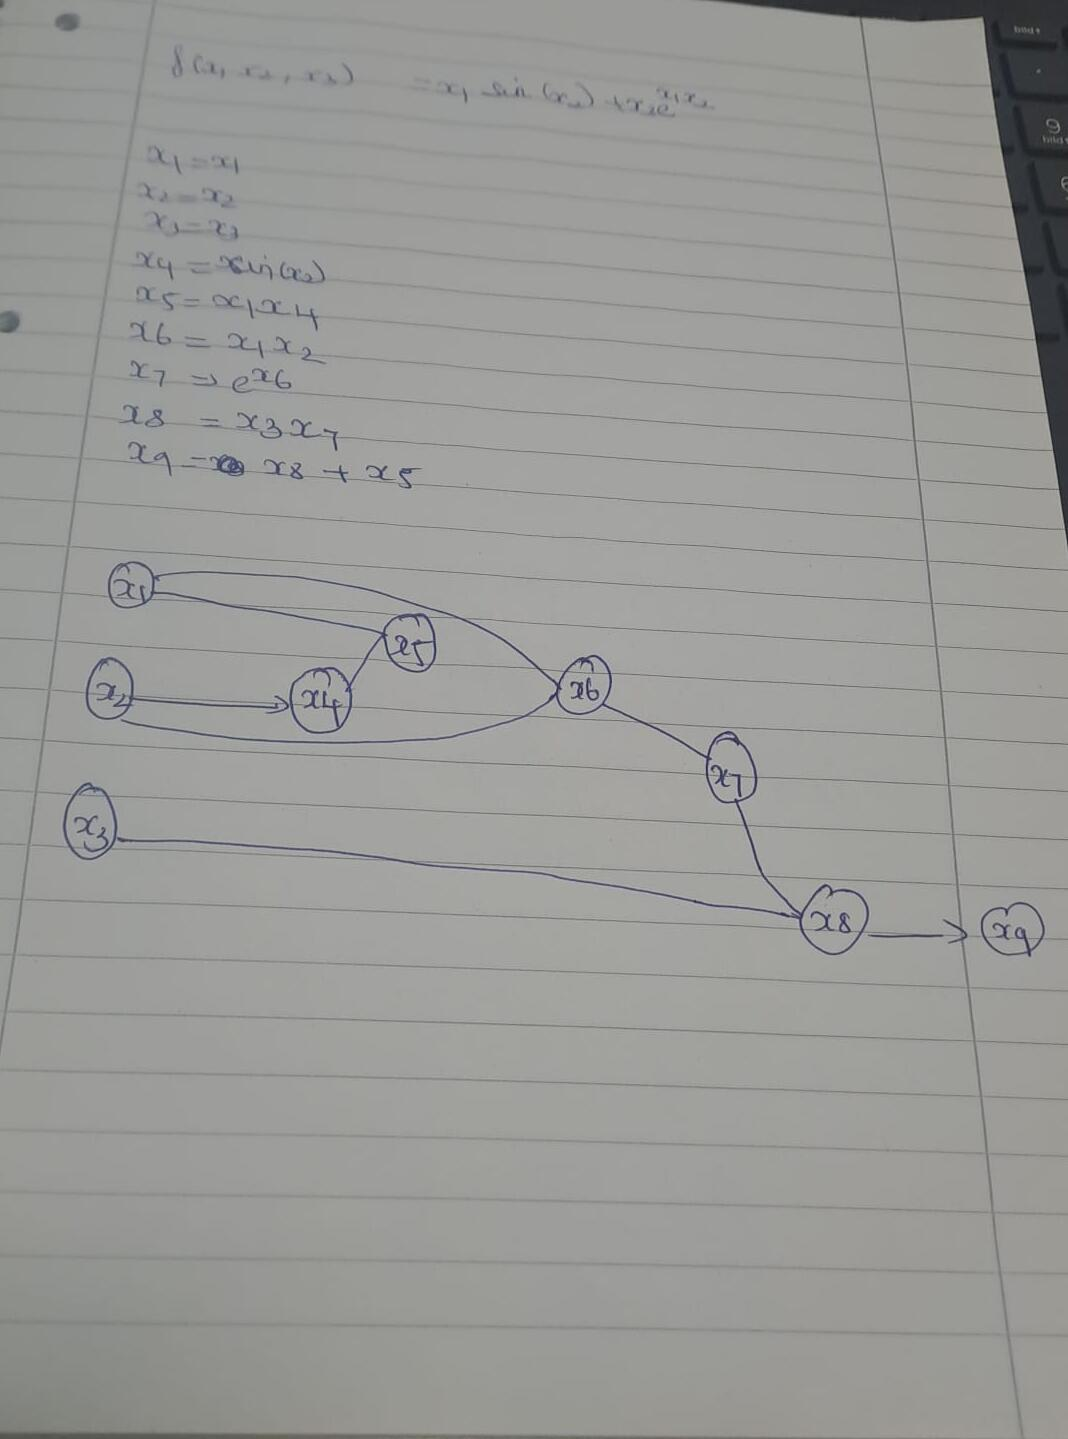
\includegraphics[width=0.8\linewidth]{images/ex3_statement.jpeg}
\end{figure}
\begin{figure}
    \centering
    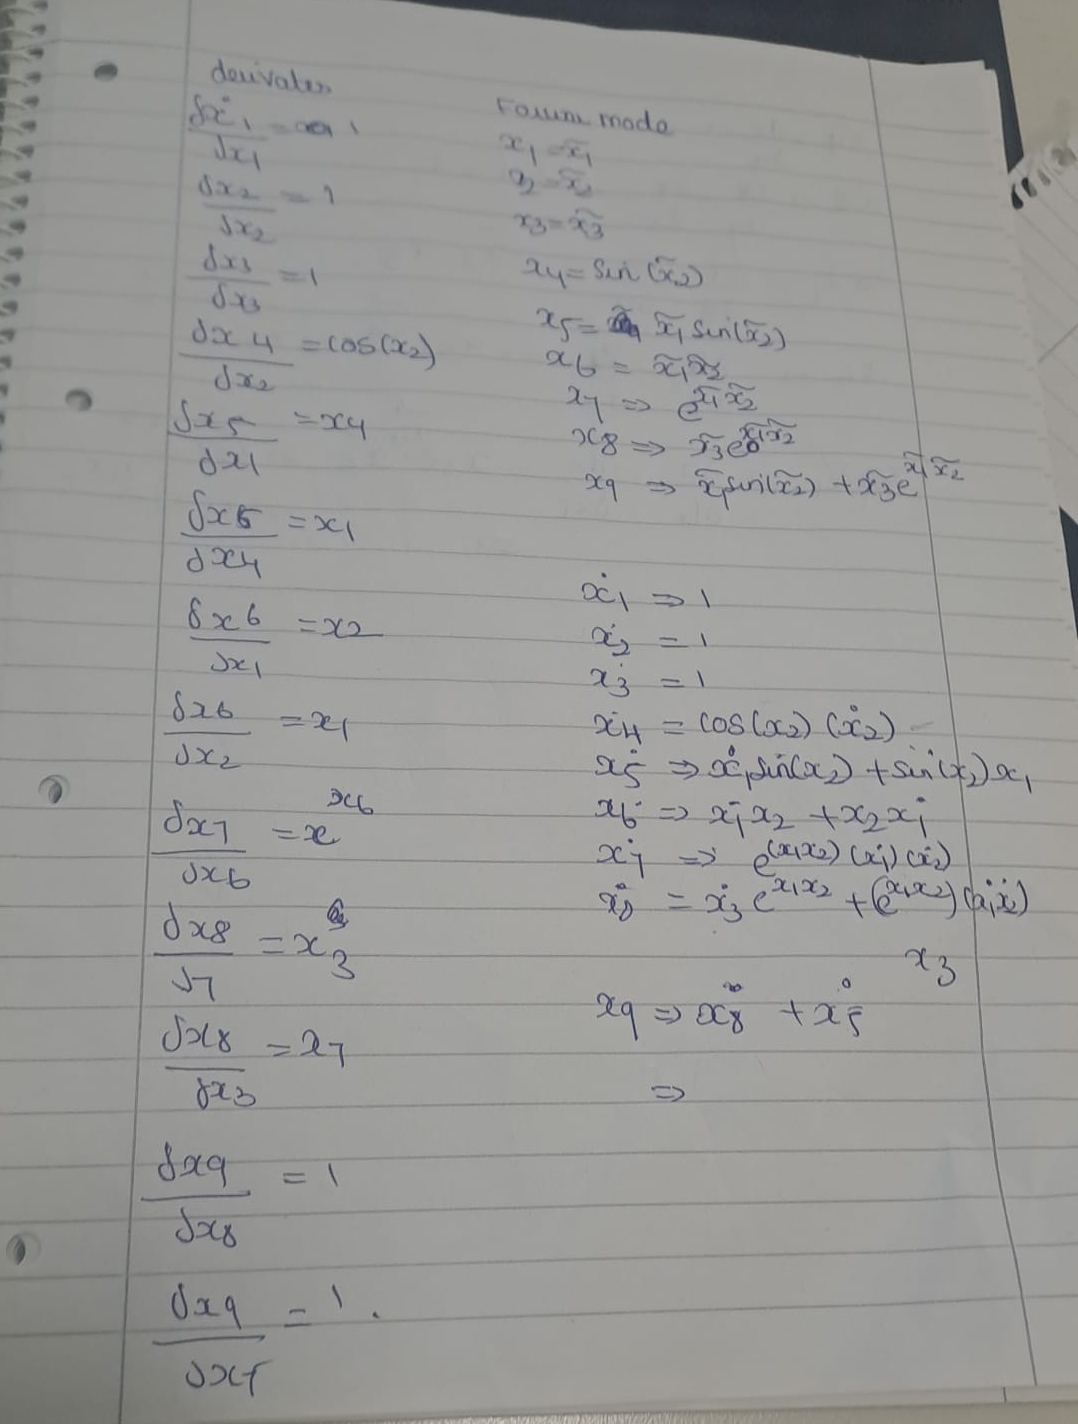
\includegraphics[width=0.8\linewidth]{images/ex3_forward_mode_1.jpeg}
\end{figure}
\begin{figure}
    \centering
    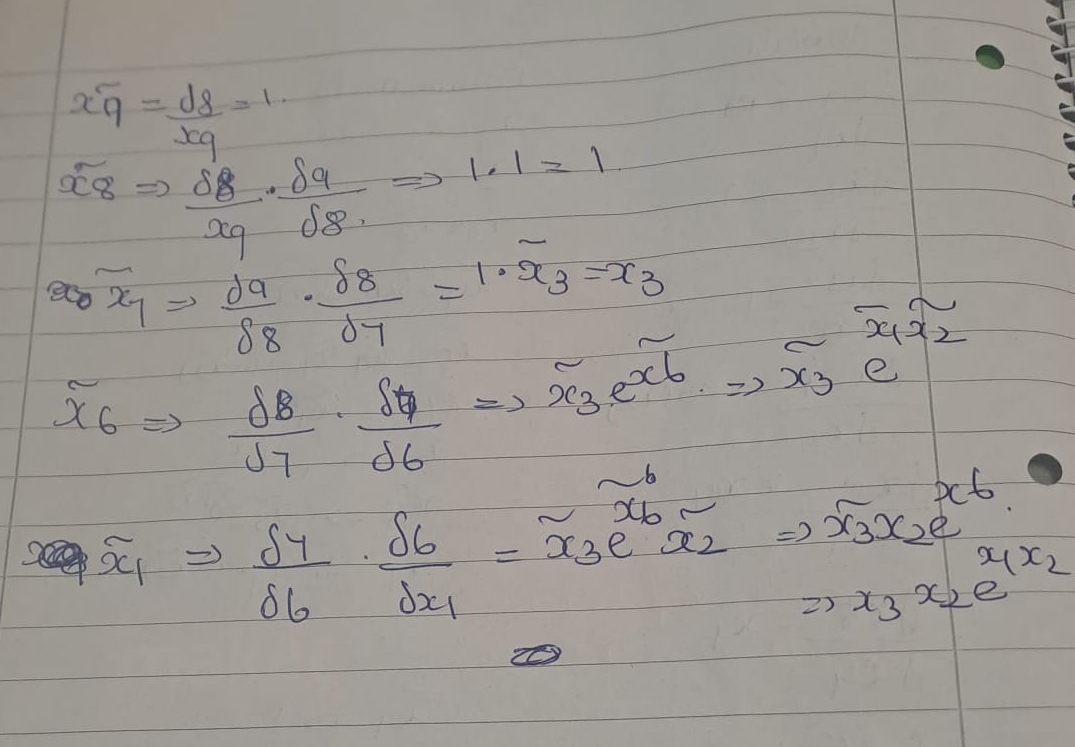
\includegraphics[width=0.8\linewidth]{images/ex3_forward_mode_2.jpeg}
\end{figure}

\end{document}
